\documentclass[color=usenames,dvipsnames]{beamer}

\mode<presentation> {

\usetheme{Madrid}

\usepackage{multirow}

\usepackage{tikz}
\usetikzlibrary{shapes.geometric, arrows}

\definecolor{ERC1}{HTML}{C72321}
\definecolor{ERC2}{HTML}{861719}
\definecolor{ERC3}{HTML}{FBD7A9}
\definecolor{ERC4}{HTML}{BA9F7C}
\definecolor{ERC5}{HTML}{7A6952}
\definecolor{ERC6}{HTML}{6E9B9E}
\definecolor{ERC7}{HTML}{0D8085}
\definecolor{ERC8}{HTML}{19484C}
\definecolor{ERC9}{HTML}{F0C320}
\definecolor{ERC10}{HTML}{AF8F19}


\tikzstyle{startstop} = [rectangle, rounded corners, minimum width=3cm, minimum height=1cm,text centered, draw=black, fill=ERC8]
\tikzstyle{io} = [trapezium, text centered, draw=white, fill=white]
\tikzstyle{process} = [rectangle, minimum width=3cm, minimum height=1cm, text centered, draw=black, fill=ERC9]
\tikzstyle{decision} = [diamond, minimum width=3cm, minimum height=1cm, text centered, draw=black, fill=ERC10]
\tikzstyle{arrow} = [thick,->,>=stealth]


\setbeamercolor{palette primary}{bg=ERC1,fg=white}
\setbeamercolor{palette secondary}{bg=ERC2,fg=white}
\setbeamercolor{palette tertiary}{bg=ERC3,fg=white}
\setbeamercolor{palette quaternary}{bg=ERC4,fg=white}
\setbeamercolor{structure}{fg=ERC5} % itemize, enumerate, etc
\setbeamercolor{section in toc}{fg=ERC6} % TOC sections


\usepackage{hyperref}
\hypersetup{%
	colorlinks=true,% hyperlinks will be coloured
	allcolors=ERC7
}



%gets rid of bottom navigation bars
\setbeamertemplate{footline}[frame number]{}

%gets rid of bottom navigation symbols
\setbeamertemplate{navigation symbols}{}

%gets rid of footer
%will override 'frame number' instruction above
%comment out to revert to previous/default definitions
\setbeamertemplate{footline}{}

% Override palette coloring with secondary
%\setbeamercolor{subsection in head/foot}{bg=UBCgrey,fg=white}


%\usecolortheme{lily}
\useoutertheme{infolines}

}


\usepackage{booktabs} 
\usepackage{tikz}


% Thin fonts
\usepackage{cmbright}
\usepackage[T1]{fontenc}

\definecolor{dark_grey}{gray}{0.5}
%\setbeamercolor{normal text}{fg=dark_grey,bg=white}
\setbeamertemplate{navigation symbols}{}

%\setbeamercolor*{palette primary}{fg=gray!100,bg=gray!10}
%\setbeamercolor*{palette quaternary}{fg=gray!100,bg=gray!10}
%\setbeamercolor*{palette secondary}{fg=gray!100,bg=gray!20}
%\setbeamercolor*{palette tertiary}{fg=gray!100,bg=gray!10}
%\setbeamercolor*{navigation symbols}{fg=white,bg=white}
\usefonttheme{default}


\setbeamertemplate{blocks}[rounded][shadow=false]
%\setbeamercolor{block title}{bg=gray!10}
%\setbeamercolor{block body}{fg=gray,bg=gray!10}
%\setbeamercolor{frametitle}{fg=}

\setbeamertemplate{frametitle}[default][center]

\setbeamertemplate{itemize items}[default]
\setbeamertemplate{enumerate items}[default]

\newcommand{\F}{\mathbb{F}}

\setbeamertemplate{title page}[default][colsep=-4bp,rounded=true]

\title[Workshop - Machine Learning]{ Don't believe the hype? A hands-on introduction to machine-learning in Python - Part I}
\subtitle{Open Workshops on Computer Based Systems Modelling}

\author{Johannes Schmidt, Johann Baumgartner}
\institute{Institute for Sustainable Economic Development, BOKU, Vienna}
\date{7.05.2019}

\begin{document}

{
\usebackgroundtemplate{
 \begin{picture}(320,315)
 \hspace{6.9cm}
   
\includegraphics[width=0.7\linewidth]{../figures/refuel_logo_with_text.png}
 \end{picture}
 }


\begin{frame}

\maketitle



\end{frame}
}
% Uncomment these lines for an automatically generated outline.
%\begin{frame}{Outline}
%  \tableofcontents
%\end{frame}


\begin{frame}{Before we start}

\begin{itemize}
	\item This is an introductionary course!
	\item Repo: \href{https://github.com/joph/Machine-Learning-Workshop}{https://github.com/joph/Machine-Learning-Workshop} or \href{https://shorturl.at/KLRT4}{https://shorturl.at/KLRT4}
	\item Bring your own data - any interest?
	\item For those who visited Peter's Python and Github Class: please fill out the feedback form at \href{https://shorturl.at/pyN26}{https://shorturl.at/pyN26}
\end{itemize}

\end{frame}


\begin{frame}{Contents - Workshop}

\begin{itemize}
\item Day 1: Introduction to Machine Learning
\item Day 2: Understanding backpropagation and Neural Networks in Python
\item Day 3: An example of a practical application of Neural Networks for image recognition in Python and Reinforcement learning in Python
\item Day 4: Bring your own data!
\end{itemize}

\end{frame}


\begin{frame}{Contents - Today} 

\begin{itemize}
\item The basic concept of machine learning
\item Some examples of machine learning
\item Supervised, unsupervised, reinforcement learning: practical exercises

\item An introduction to neural networks 

\end{itemize}

\end{frame}

\begin{frame}{Main Literature}

\begin{itemize}
\item \href{https://www.coursera.org/learn/machine-learning}{{Introduction to Machine Learning by Andrew Ng (Coursera.org)}}
\item Deep Learning with Python by Francois Chollet
\end{itemize}

\end{frame}



%\vskip 1cm

%\begin{block}{Examples}
%Some examples of commonly used commands and features are included, to help you get started.
%\end{block}

\begin{frame}{Simple and hard tasks} 

Traditionally simple tasks for a computer (but hard for humans)

\begin{itemize}
	\item $\log{\sqrt{x^3+y*z^7}},x = 329$
	\item Search for all occurrences of "European Union" in a (superlong) text
	\item Generate a 3D scene from a mathematical description, using raytracing
	\item Compile a computer program	
\end{itemize}	

Traditionally hard tasks for a computer (but simple for humans)
\begin{itemize}
	\item Who is on that photo?
	\item Is this a cat or a dog?
	\item Generate a realistic image of a person
	\item Generate human readable text
	\item Translate one language to another one		
\end{itemize}	

\end{frame}

\section{The basic concept of machine learning}


\begin{frame}{The basic concept of machine learning} 


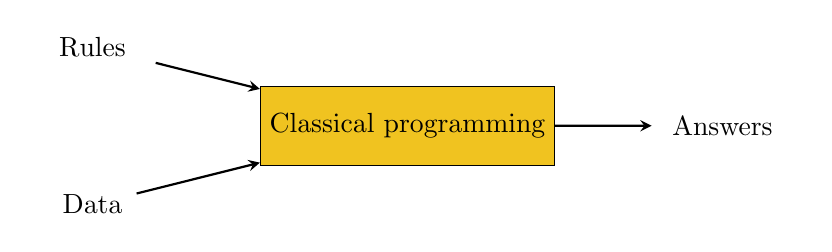
\begin{tikzpicture}[node distance=2cm]

%\node (Start) [startstop] {Start};

\node (in1) [io] {Rules};
\node (in2) [io, below of=in1] {Data};


\node (pro1) [process, right of=in1, xshift = 2cm, yshift = -1cm] {Classical programming};

\node (out1) [io, right of=pro1, xshift = 2cm] {Answers};

\draw [arrow] (in1) -- (pro1);
\draw [arrow] (in2) -- (pro1);

\draw [arrow] (pro1) -- (out1);


\end{tikzpicture}

\vspace{1cm}

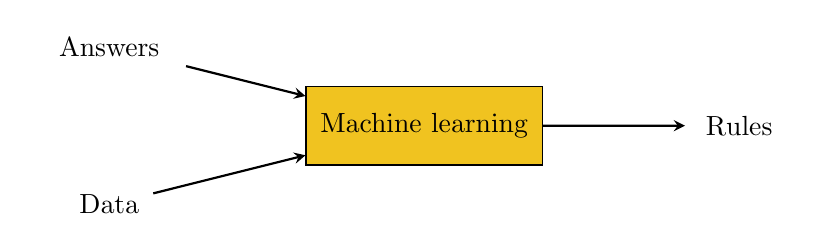
\begin{tikzpicture}[node distance=2cm]

%\node (Start) [startstop] {Start};

\node (in1) [io] {Answers};
\node (in2) [io, below of=in1] {Data};


\node (pro1) [process, right of=in1, xshift = 2cm, yshift = -1cm] {Machine learning};

\node (out1) [io, right of=pro1, xshift = 2cm] {Rules};

\draw [arrow] (in1) -- (pro1);
\draw [arrow] (in2) -- (pro1);

\draw [arrow] (pro1) -- (out1);


\end{tikzpicture}



%\vskip 1cm

%\begin{block}{Examples}
%Some examples of commonly used commands and features are included, to help you get started.
%\end{block}

\end{frame}

\begin{frame}{Why is this cool or frightening?} 


\begin{itemize}

\item \href{https://www.captionbot.ai/}{{Image recognition with captionbot.ai}}

\item \href{https://www.youtube.com/watch?time_continue=2&v=TmPfTpjtdgg}{{Computer plays Atari computer games}}


%	\item \href{https://youtu.be/rOL6QJdAlm8?t=103}{{The moment alphaGo wins against Lee Sedol}}

\item \href{https://www.thispersondoesnotexist.com/}{{This person does not exist}}

\item \href{https://www.newscientist.com/article/2186512-exclusive-uk-police-wants-ai-to-stop-violent-crime-before-it-happens/}{{Minority report}}

\item \href{https://dishtracker.at/?lang=de}{{Supervising Oktoberfest waiters}}

\item \href{https://link.springer.com/book/10.1007/978-3-030-16800-1}{{Write a (boring) book}}

\item \href{https://www.theverge.com/2019/4/25/18516004/amazon-warehouse-fulfillment-centers-productivity-firing-terminations}{{Amazon automatically tracks and fires warehouse workers} }

\item \href{https://gizmodo.com/an-ai-lie-detector-is-going-to-start-questioning-travel-1830126881}{{AI Lie detector for border control}}

\item \href{https://twitter.com/oe1/status/1119239287541833728?s=08}{{Twitter content filter going wrong}}

\item \href{https://futurezone.at/netzpolitik/computer-sagt-nein-algorithmus-gibt-frauen-weniger-chancen-beim-ams/400345297}{{ Arbeitsmarktservice predicts probability of finding a job}}

\end{itemize}

\end{frame}

\section{Terminology}


\begin{frame}{A typology of machine learning} 


\begin{itemize}

\item Supervised learning: Given inputs and outputs, find the rules that link the two
\item Unsupervised learning: Find structure in data
\item Reinforcement learning: learning by doing

\end{itemize}

\end{frame}

\begin{frame}{Supervised learning - Exercise (I)} 



\begin{table}[ht]
\centering
\begin{tabular}{c|c}
Positives&Negatives\\
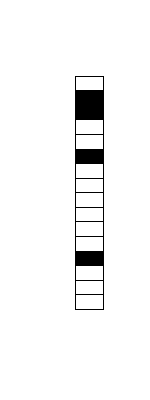
\includegraphics[width=0.1\linewidth]{../figures/1d_pattern_supervised_learning_1.png}
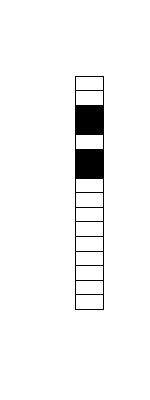
\includegraphics[width=0.1\linewidth]{../figures/1d_pattern_supervised_learning_2.png}
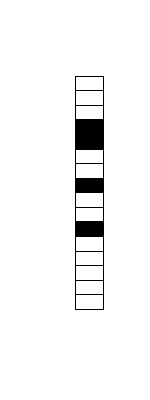
\includegraphics[width=0.1\linewidth]{../figures/1d_pattern_supervised_learning_3.png}
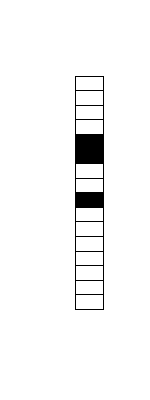
\includegraphics[width=0.1\linewidth]{../figures/1d_pattern_supervised_learning_4.png}&
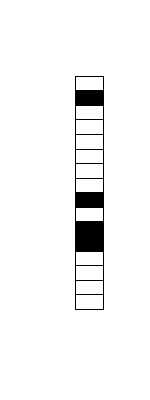
\includegraphics[width=0.1\linewidth]{../figures/1d_random_supervised_learning_1.png}
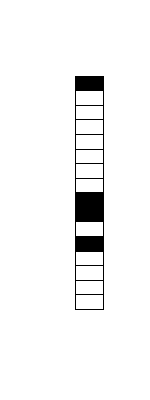
\includegraphics[width=0.1\linewidth]{../figures/1d_random_supervised_learning_2.png}
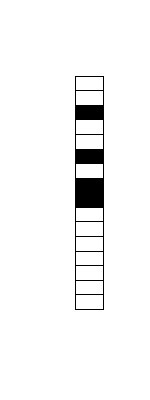
\includegraphics[width=0.1\linewidth]{../figures/1d_random_supervised_learning_3.png}
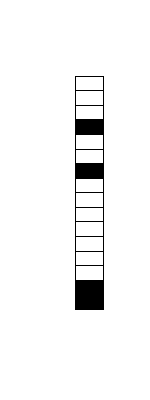
\includegraphics[width=0.1\linewidth]{../figures/1d_random_supervised_learning_4.png}
\\
\end{tabular}
\end{table}

\begin{center}
Positive or Negative?\\
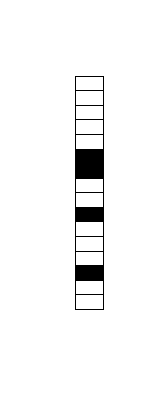
\includegraphics[width=0.1\linewidth]{../figures/1d_pattern_supervised_learning_5.png}
\end{center}

\end{frame}


\begin{frame}{Supervised learning needs labeled datasets} 

\begin{itemize}
\item Classification. Input features: Photos of people. Labels: smiling or not.
\item Classification. Input features: Photos of waiters carrying plates and glasses. Labels: number of plates and glasses.
\item Classification. Input features: German text. Labels: English text.
\item Regression. Input features: wind speeds. Labels: measured wind power generation.
\item Therefore: 
\href{https://www.theverge.com/2019/3/28/18285572/prison-labor-finland-artificial-intelligence-data-tagging-vainu}{{Inmates in Finland are training AI as part of prison labor}}
\end{itemize}

\end{frame}


\begin{frame}{Unsupervised learning - Exercise} 

\begin{center}
Which data points belong to each other?\\
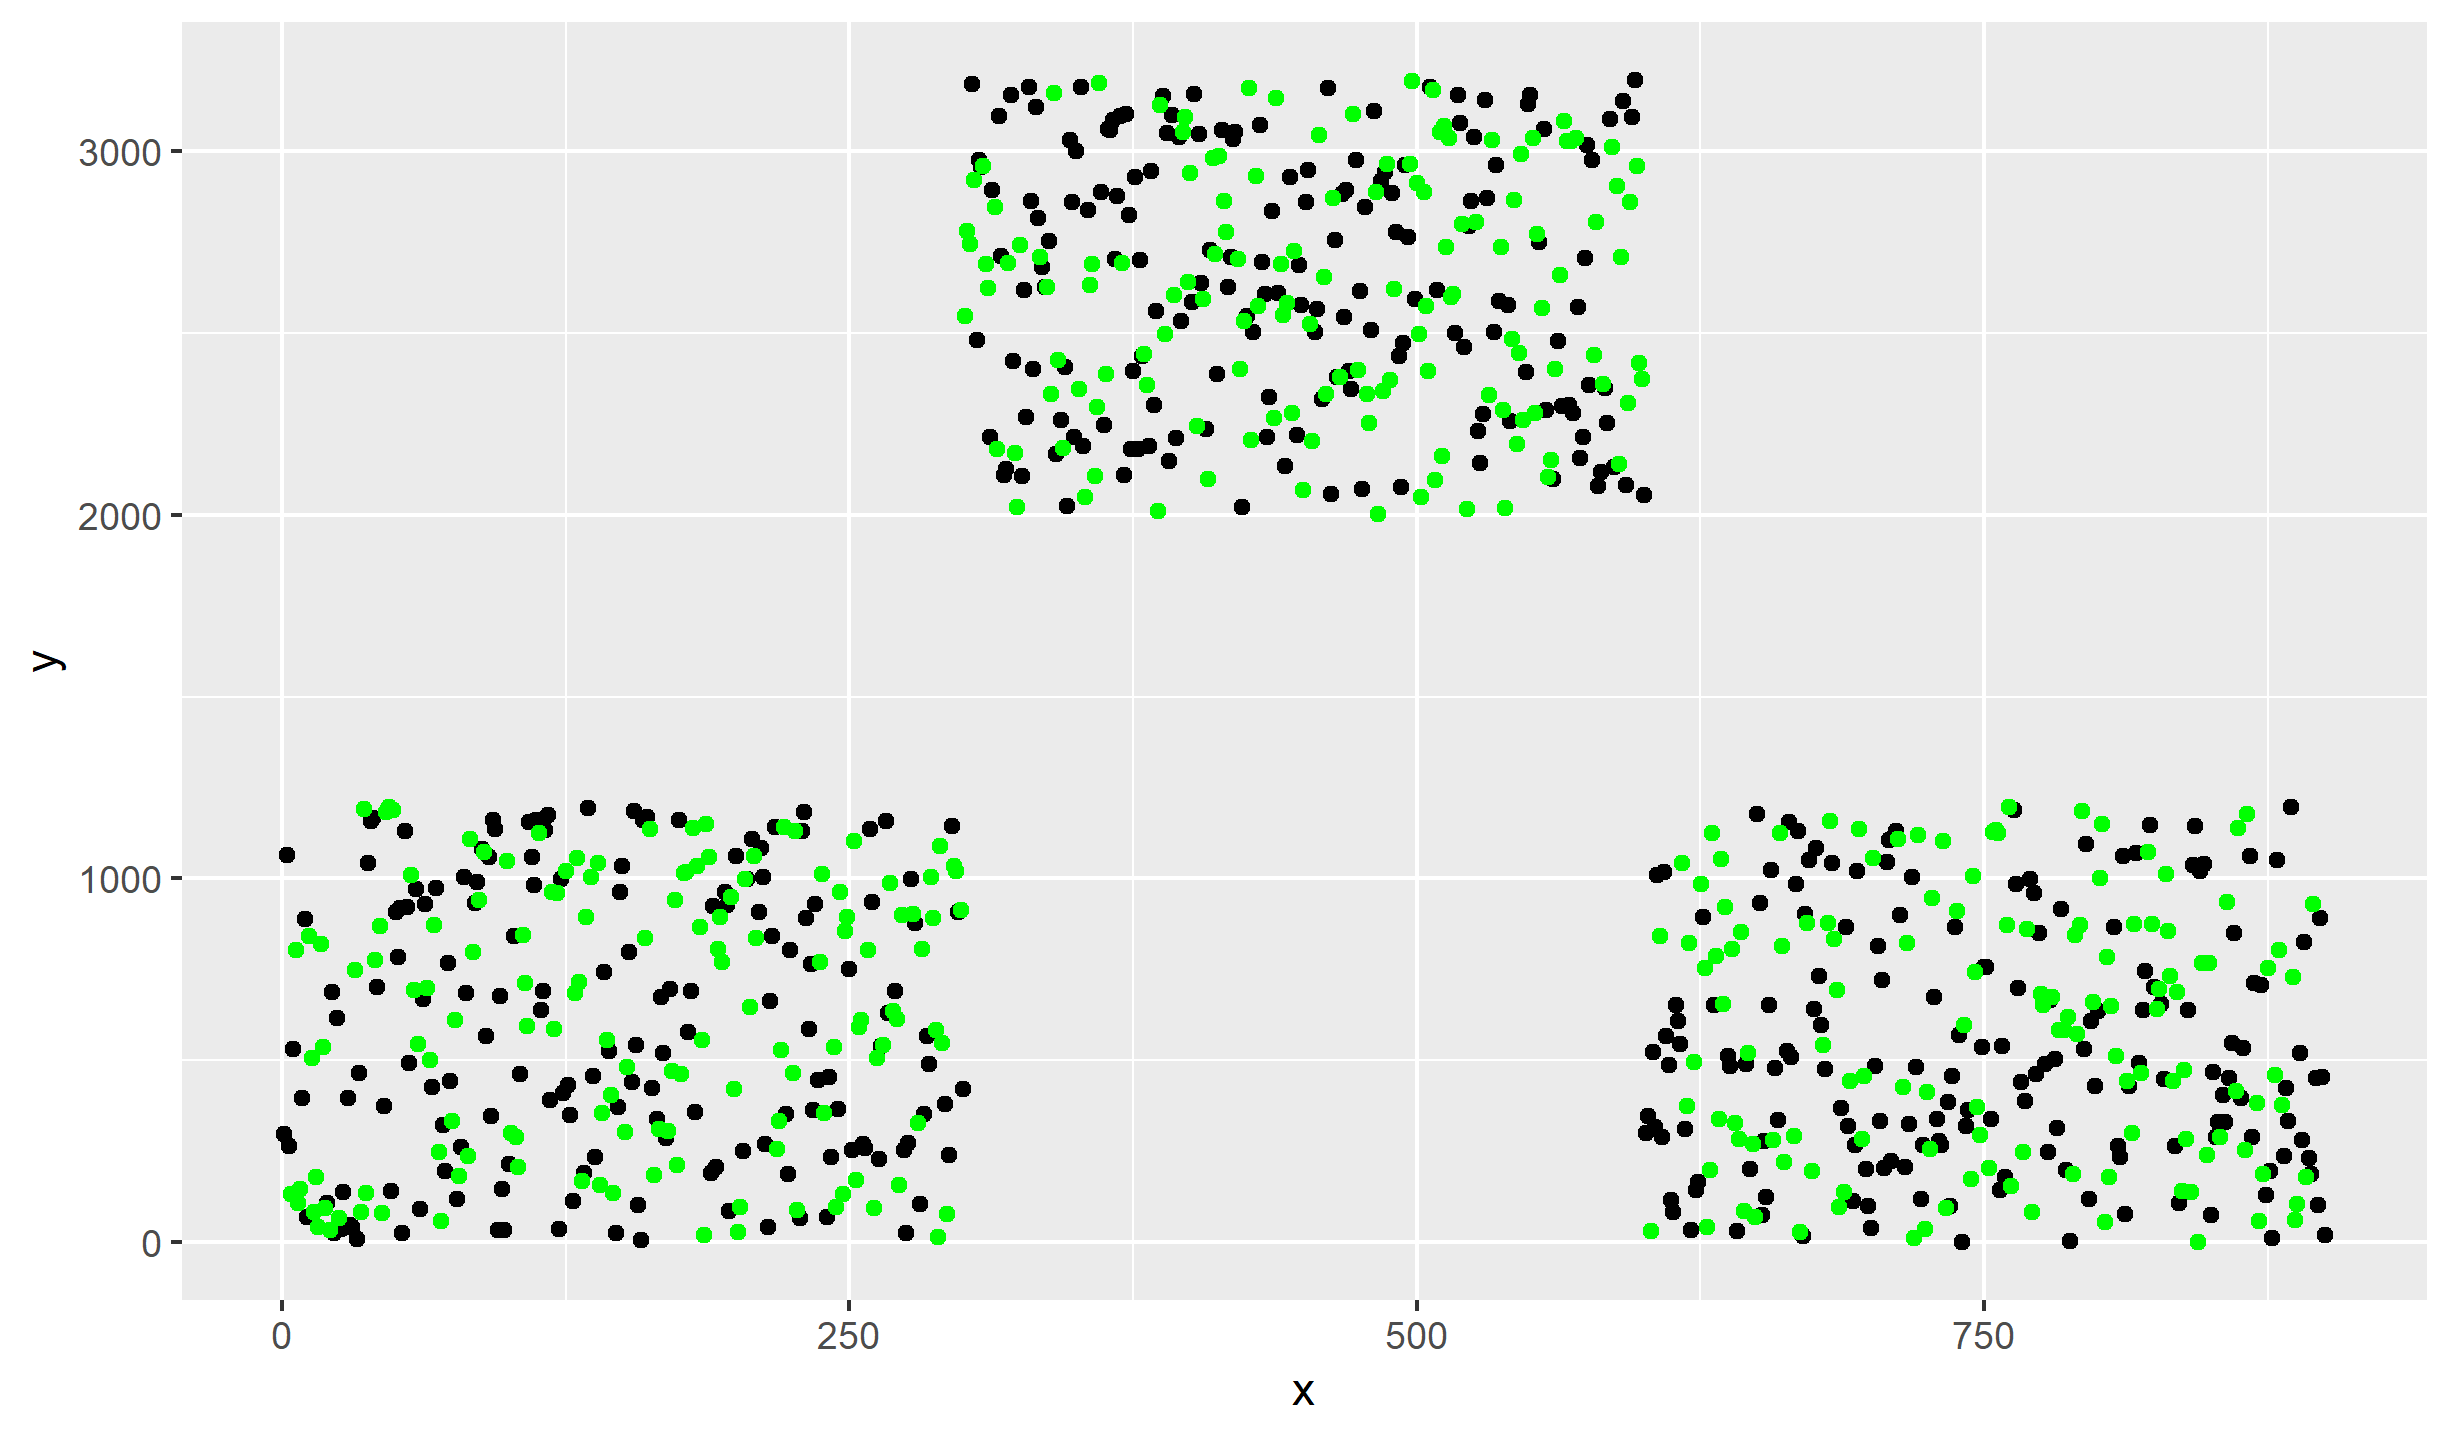
\includegraphics[width=0.8\linewidth]{../figures/clustering.png}
\end{center}


\end{frame}

\begin{frame}{Unsupervised learning - Find structure in data} 

\begin{itemize}
\item Clustering (which data belongs together?)
\item Anomaly detection (which data is somehow strange?)
\item Generative adversial networks (Generate photos, sounds, and text, also involves supervised learning)
\end{itemize}

\end{frame}


\begin{frame}{Reinforcement learning - Exercise} 

See Netlogo

\end{frame}

\begin{frame}{Reinforcement learning - Learning by doing} 

\begin{itemize}
\item Propose new videos on video platform to user
\item Play Computer Games or Go
\item Simulation of heuristic optimization of agents (e.g. on markets)
\end{itemize}

\end{frame}

\begin{frame}{What is it?} 

\begin{itemize}
\item Google translate
\item Amazon product suggestion
\item Face recognition
\item Facebook face recognition
\item \href{https://arxiv.org/pdf/1802.09756.pdf}{{Bidding for advertisements on Taobao}}
\end{itemize}

\end{frame}

\begin{frame}{An introduction to artificial neural networks} 

\begin{itemize}
\item Why neural networks?
\item Basic concepts and terminology
\item Backpropagation algorithm and its computational complexity
\item Under- and overfitting of neural networks
\item Practical aspects of machine learning
\end{itemize}

\end{frame}


\begin{frame}{Why artificial neural networks?} 

\begin{itemize}
\item Current state of the art in pattern recognition, and language processing
\item Used in supervised learning, unsupervised learning, and reinforcement learning
\item Understanding neural networks will help you to understand other algorithms too

\end{itemize}

\end{frame}

\begin{frame}{Are they new?} 

\begin{itemize}
\item \href{https://scholar.google.at/citations?user=tvUH3WMAAAAJ&hl=de}{{Well... not really}}
\item 1940ies first work
\item Short lived hypes in 60ies and 80ies
\item 1997: US Mail uses ANNs for recognizing handwritten addresses
\item New hype starting around 2010
\end{itemize}

\end{frame}


\begin{frame}{What are they used for?} 

\begin{itemize}
\item Classification
\item Regression
\item Text and Image generation
\item Anything, that needs the approximation of a function
\end{itemize}

\end{frame}

\begin{frame}{Wait... regression? Classification?} 

You've heart it before, but no ANNs were involved? Well, ordinary least squares regression is around since the 19th century.\\

Ok, so what's the difference?\\

\begin{itemize}
\item Ordinary Least Squares regression needs assumptions on functional relationships. (blackboard example)
\item In contrast, ANNs are \textit{Universal Function Approximators} for linear, bounded functions. You don't have to specify functional relationships. For a nice visual proof of it, see \href{http://neuralnetworksanddeeplearning.com/chap4.html} {{here}}
\item ANNs \textbf{do not} allow deriving impact of input parameters on output (such as statistical significance)
\item ANNs are therefore useful for prediction, but not for statistical inference
\item Machine learning uses way cooler vocabulary
\end{itemize} 

\end{frame}

\begin{frame}{Universal Function Approximator?} 


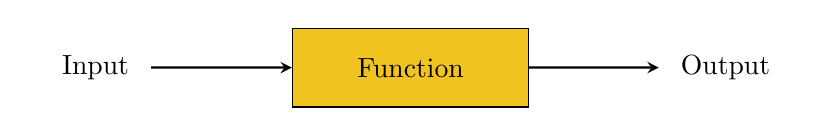
\begin{tikzpicture}[node distance=2cm]

%\node (Start) [startstop] {Start};

\node (in1) [io] {Input};

\node (pro1) [process, right of=in1, xshift = 2cm] {Function};

\node (out1) [io, right of=pro1, xshift = 2cm] {Output};

\draw [arrow] (in1) -- (pro1);
\draw [arrow] (pro1) -- (out1);


\end{tikzpicture}
\vspace{1cm}

Possible Input Output relations
\begin{itemize}
\item German Language -> English Language
\item Photos of cats and dogs -> Classification "Cat", "Dog"
\item x -> $x^2$
\item Weather data -> Wind power generation	
\end{itemize}

\end{frame}

\begin{frame}{Elephants} 

Wait... but what about "With four parameters I can fit an elephant, and with five I can make him wiggle his trunk." (John von Neumann)\\


\begin{center}
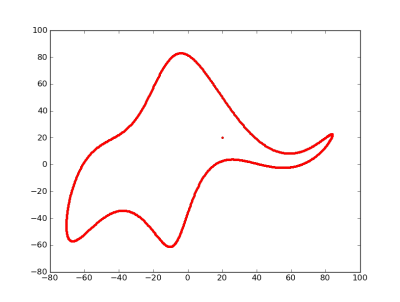
\includegraphics[width=0.5\linewidth]{../figures/elephant.png}\\

\href{https://www.johndcook.com/blog/2011/06/21/how-to-fit-an-elephant/}{{Fit the elephant in python with four complex numbers}}

\end{center}

So true: the art of ANNs lies in achieving reasonable fits without \textbf{overfitting}.\\ 

\end{frame}


\begin{frame}{Basic terminology} 

\begin{itemize}
\item Input layer (features)
\item Hidden layer
\item Output layer (labels)
\item Nodes
\item Connections
\item Weights
\item Bias node
\item Activation function
\item Error measure
\end{itemize}

\end{frame}





\begin{frame}{Backpropagation algorithm} 

\begin{itemize}
\item Weights are adapted, so that the prediction and the observation error is minimized.\\
\item Non-convex optimization due to non-convex activation functions: heuristic approach\\
\item \href{https://page.mi.fu-berlin.de/rojas/neural/chapter/K10.pdf}{{Training neural networks is NP-Complete in its most general form.}}\\
\item \href{https://mattmazur.com/2015/03/17/a-step-by-step-backpropagation-example/}{An example calculation}

\end{itemize}

\end{frame}

\begin{frame}{Terminology data sets and training} 

\begin{itemize}
\item Sample
\item Training data
\item Validation data 
\item Test data
\item Epoch
\item Batch, batch size
\item Online training, micro-batch training, batch training
\end{itemize}

\end{frame}

\begin{frame}{Underfitting}

\begin{itemize}
\item Both training and validation data do not fit well.
\item Problem: not enough data to fit to your network
\item Solution: Smaller network. Or more data.
\end{itemize}

\end{frame}




\begin{frame}{Overfitting}

\begin{itemize}
\item Training data fits well, validation or test data does not. 
\item Problem: Network is adapted perfectly to your training data, but does not generalize.
\item Solution: larger network. Add leaky ReLu layers. 
\end{itemize}

\end{frame}

\begin{frame}{Out of range}

Never forget: ANNs are universal function approximators for \textbf{bounded regions}.
\end{frame}



\begin{frame}{Practical aspects} 

\begin{itemize}
\item Always assess variance-bias trade-off to understand under- and overfitting
\item Get a GPU!
\item Play around (get a GPU!)
\item Choose your problems wisely. (If OLS regression works, use it, it gives much more insights.)
\item Use feature engineering. With and without neural networks.
\end{itemize}

\end{frame}

\begin{frame}{Next workshops} 

What we do
\begin{itemize}

\item Neural Networks – Overview of types
\item Suitability of types to problems
\item How does backpropagation work?
\item Build intuition of inner workings of neural networks – netlogo model
\item Keras Neural network sequential model vs api
\item Building blocks of a keras neural networks
\item Neural network training and prediction (incl. wind power generation example)
\item Hyperparameter optimization and steps forward
\end{itemize}

What to bring
\begin{itemize}
\item A laptop
\item Python installed with the following packages: keras, scikit-learn
\item Netlogo installed
\end{itemize}

\end{frame}

{
\usebackgroundtemplate{
\begin{picture}(320,315)
\hspace{6.9cm}

\includegraphics[width=0.7\linewidth]{../figures/refuel_logo_with_text.png}
\end{picture}
}


\begin{frame}
\frametitle{Thank you!}
\begin{block}{
For slides and source-code, check \textbf{https://github.com/joph/Machine-Learning-Workshop}\\
mail: johannes.schmidt@boku.ac.at\\

}
\end{block}

\vspace{2.5 cm}


\end{frame}

}








\end{document} 